% This is samplepaper.tex, a sample chapter demonstrating the
% LLNCS macro package for Springer Computer Science proceedings;
% Version 2.20 of 2017/10/04
%
\documentclass[runningheads]{llncs}
%
\usepackage{graphicx}

%Paquetes añadidos
\usepackage{float}
\usepackage{subcaption}
\captionsetup{compatibility=false}

% Used for displaying a sample figure. If possible, figure files should
% be included in EPS format.
%
% If you use the hyperref package, please uncomment the following line
% to display URLs in blue roman font according to Springer's eBook style:
% \renewcommand\UrlFont{\color{blue}\rmfamily}

\begin{document}
	%
	\title{Bibliographic work\thanks{Supported by organization x.}}
	%
	%\titlerunning{Abbreviated paper title}
	% If the paper title is too long for the running head, you can set
	% an abbreviated paper title here
	%
	\author{Erik Cembreros\inst{1}\orcidID{0000-1111-2222-3333} \and
		Josu Barrutia\inst{2,3}\orcidID{1111-2222-3333-4444} \and
		Third Author\inst{3}\orcidID{2222--3333-4444-5555}}
	%
	\authorrunning{F. Author et al.}
	% First names are abbreviated in the running head.
	% If there are more than two authors, 'et al.' is used.
	%
	\institute{Princeton University, Princeton NJ 08544, USA \and
		Springer Heidelberg, Tiergartenstr. 17, 69121 Heidelberg, Germany
		\email{lncs@springer.com}\\
		\url{http://www.springer.com/gp/computer-science/lncs} \and
		ABC Institute, Rupert-Karls-University Heidelberg, Heidelberg, Germany\\
		\email{\{abc,lncs\}@uni-heidelberg.de}}
	%
	\maketitle              % typeset the header of the contribution
	%
	\begin{abstract}
			
		
		\keywords{First keyword  \and Second keyword \and Another keyword.}
	\end{abstract}
	%
	%
	%
	
	\clearpage
	\section{Results analysis}
	
	Five prespecified access point topologies have been considered to compare how do they affect the placement and movement trends of the jammers. To achieve this the simplified bilevel mixed-
	integer program [BLMIP] has been used.
	
	The Partite topology had three clusters with demand points clustering around them. The Perimeter topology distributed access points along the region's perimeter, allowing free movement of demand points. The Dense topology featured a central hub with clustered access points, catering to high demand independently. The Spacious topology randomly distributed access points to avoid proximity, resulting in demand points within range of one or two access points. The Median topology had uniformly distributed access points along diagonals and central lines, with clustering in the center, resembling a campus with a central area of high connectivity demand. It also includes an optimal topology, generated from solving one problem instance.
	
\begin{figure}[H]
	\centering
	\begin{subfigure}{0.3\textwidth}
		\centering
		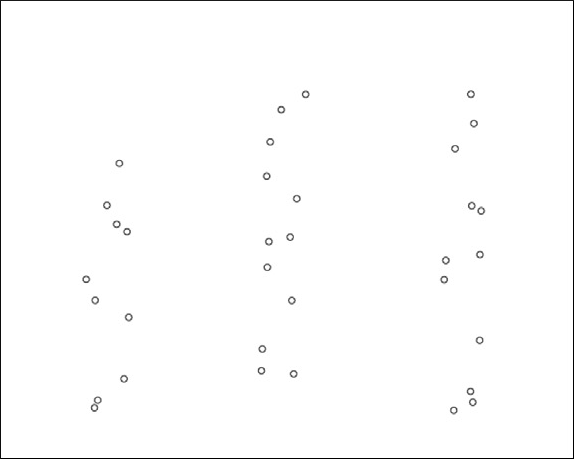
\includegraphics[width=.8\linewidth]{partite.png}\quad
		\caption{Partite}
		\label{fig:1}
	\end{subfigure}\hfil
	\begin{subfigure}{0.3\textwidth}
		\centering
		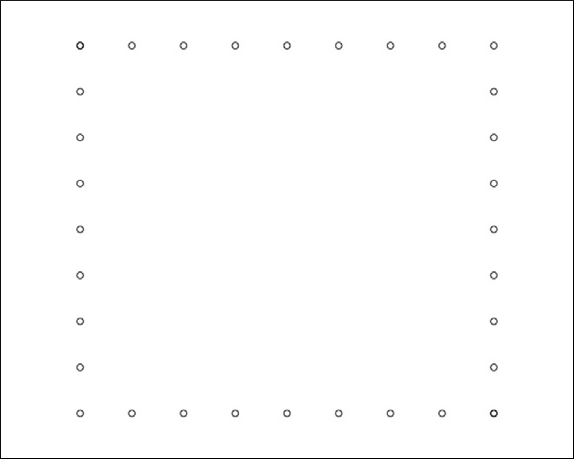
\includegraphics[width=.8\linewidth]{perimeter.png}\quad
		\caption{Perimeter}
		\label{fig:2}
	\end{subfigure}\hfil
	\begin{subfigure}{0.3\textwidth}
		\centering
		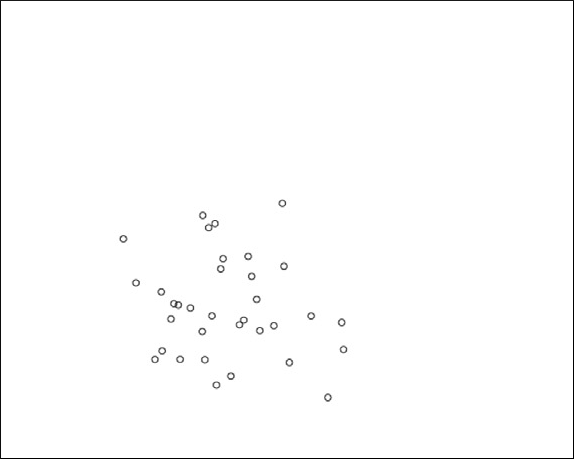
\includegraphics[width=.8\linewidth]{dense.png}
		\caption{Dense}
		\label{fig:3}
	\end{subfigure}
	\medskip
	\begin{subfigure}{0.3\textwidth}
		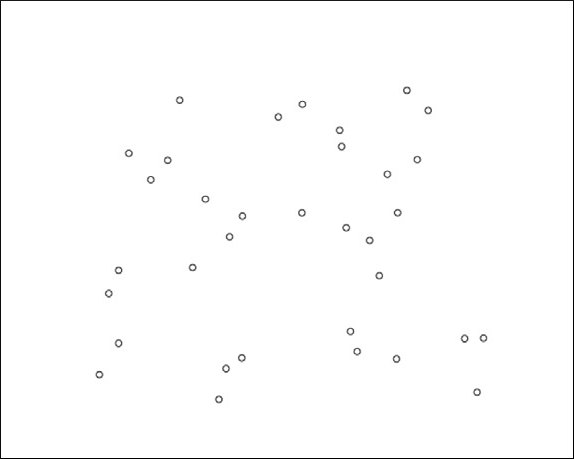
\includegraphics[width=.8\linewidth]{spacious.png}\quad
		\caption{Spacious}
		\label{fig:4}
	\end{subfigure}\hfil
	\begin{subfigure}{0.3\textwidth}
		\centering
		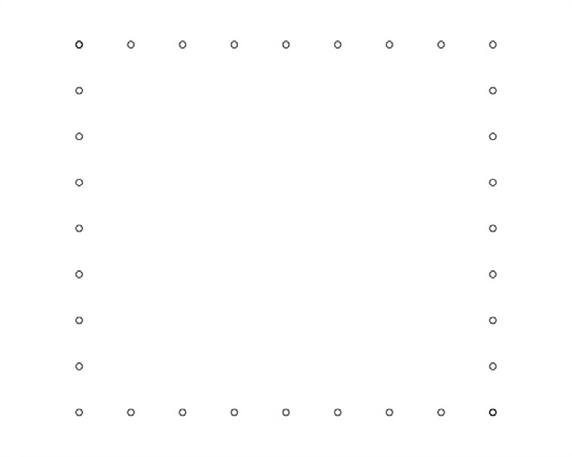
\includegraphics[width=.8\linewidth]{median.png}\quad
		\caption{Median}
		\label{fig:5}
	\end{subfigure}\hfil
	\begin{subfigure}{0.3\textwidth}
		\centering
		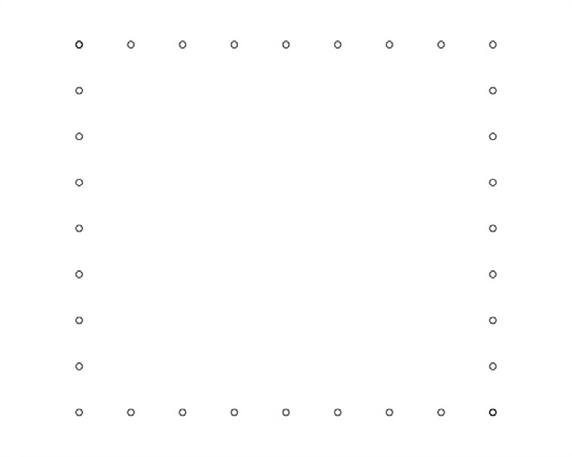
\includegraphics[width=.8\linewidth]{optimal.png}
		\caption{Optimal}
		\label{fig:6}
	\end{subfigure}
	\caption{AP Topologies}
	\label{fig:images}
\end{figure}
	
	
	For all five topologies, three experiments with 10, 25 and 50 AP, each with a capacity of 15, 5 jammers with jamming radius of 150 feet, and 5 time periods. Each region was 1 square mile. The demand was realized ten times, with 100 demand points, and the results were averaged.
	
	
	Attending to the non-additive model, two methodologies were used to examine the runtime solutions: branch-and-bound and implicit enumeration. The latter algorithm significantly outperformed the first one. Whereas for the additive model, the implicit enumeration fared better than branch-and-bound, without dynamically generated covers. The introduction of dynamically generated covers had a significant positive impact on the overall computational speed. When applied exclusively to the branch-and-bound algorithm, the inclusion of dynamically generated covers yielded only marginal improvements compared to the basic implicit enumeration algorithm. 
	
	It was found that access point placement near concentrations of demand points was crucial for ensuring robust network connectivity. However, access points too clustered together give jammers an easier time on severing connections. Therefore, the optimal solution should find a balance between these two factors. The Spacious topology demonstrated the closest resemblance to the optimal access point placement, suggesting a high likelihood of establishing and maintaining connections. The non-additive model consistently yielded weaker results, except in the Partite topology, which exhibited clustering. In contrast, the additive model prioritized connections close to jammers, and the presence of access point clusters implied more effective access-demand point connections in proximity to jammers. When directly comparing the additive and non-additive models, significant relative errors were observed across all topologies, with the Dense and Median topologies showing the largest discrepancies due to the clustering of demand points.
	
	Sensitivity has also been proved, concluding that adding a set of new access points did not improve overall connectivity. Meanwhile, were more jammers to be added to the original problem, the set of new APs would become significantly important.
	
	\ref{Eq3a} is a generalized utility function considering three aspects: range, unity and tolerance.
	The range describes signal strength for access-demand point connections, unity represents uniform signal strength with either connected or unconnected links and tolerance introduces a threshold below which connections are considered too weak to be useful and are treated as unconnected.
	
	
	
	\section{Conclusions}
	
	The optimal placement of access points is crucial to ensure maximum connectivity for demand points in various environments, such as university campuses. This optimal topology will also maximize connectivity in the presence of jammers, considering both non-additive and additive models.
	The key for a proper placement is to strike a balance between placing access points near concentrations of demand points and avoiding the formation of clusters.	The Partite and Median topologies demonstrated greater robustness against jamming attacks when considering utility as total signal strength, number of connections, or tolerance allowance.
	
	In this research, both the placement of access points and jammers have been considered, but not the placement of demand points. Considering this would lead to a stochastic problem rather than a deterministic one.
	
	
	%
	% ---- Bibliography ----
	%
	% BibTeX users should specify bibliography style 'splncs04'.
	% References will then be sorted and formatted in the correct style.
	%
	% \bibliographystyle{splncs04}
	% \bibliography{mybibliography}
	%
	\begin{thebibliography}{8}
		\bibitem{ref_article1}
		Author, F.: Article title. Journal \textbf{2}(5), 99--110 (2016)
		
	\end{thebibliography}
\end{document}

